% !TEX encoding = UTF-8 Unicode
\documentclass[9pt, oneside]{extarticle}   	% use for two column: ,twocolumn
\usepackage{hyperref}
\usepackage{fancyvrb}
	\fvset{tabsize=4}%changes tab spacing in verbatim from 8 to 4
%\usepackage{geometry}                		% See geometry.pdf to learn the layout options. There are lots.
%\geometry{letterpaper}                   		% ... or a4paper or a5paper or ...
%\usepackage[pass,letterpaper]{geometry}
\usepackage[margin=2cm,letterpaper]{geometry}
%\geometry{landscape}                		% Activate for for rotated page geometry
\usepackage[parfill]{parskip}    		% Activate to begin paragraphs with an empty line rather than an indent
\usepackage{graphicx}				% Use pdf, png, jpg, or eps? with pdflatex; use eps in DVI mode
									% TeX will automatically convert eps --> pdf in pdflatex
\usepackage{amssymb}
\usepackage{tikz,adjust box}			%adjustbox is for figures that span 2 columns
\usepackage{dashrule}				%used to make dashed line in text
\usepackage{amsmath}
\usepackage{fancyhdr}				%used to put draft in header
%\pagestyle{fancy}					%
\DeclareMathOperator{\arcsec}{arcsec}	%arcsec, arccsc... not defined inamsmath
\usepackage{exsheets}				%Formats questions and solutions
\SetupExSheets{solution/print=false,question/name={},solution/name={}}		%Solutions on or off;
\SetupExSheets{headings=runin}		% Puts questions next to number
\SetupExSheets{use-classes={easy,medium,hard}}	% Print questions by difficulty level
\usepackage{natbib,endnotes}			%Bibliography and Footnote to endnote
\usepackage{title sec}				%Format section titles to include horizontal line
%\usepackage{enumitem}				%Allow lists to be a, b, c and not 1, 2, 3
\usepackage{enumerate}
\usepackage{epigraph}




%\renewcommand{\theenumi}{\alph{enumi}}
%\setenumerate[0]{label=(\alph*)}
\let\footnote\endnote
\titleformat{\section}
  {\normalfont\Large\bfseries}{\thesection}{1em}{}[{\titlerule[0.8pt]}]
\newcommand{\calc}{\protect\includegraphics[height = 2.5ex]{images/calc.png}}
%%%%%%%%%%%%%%%%%%%%%%%%%%%%%%%%%%%%%%%%%%%%
%%%%%%%%Convert paragraph to subsubsubsection %%%%%%%%%%%%%%%%
\makeatletter
\renewcommand\paragraph{\@startsection{paragraph}{4}{\z@}%
            {-2.5ex\@plus -1ex \@minus -.25ex}%
            {1.25ex \@plus .25ex}%
            {\normalfont\normalsize\bfseries}}
\makeatother
\setcounter{secnumdepth}{4} % how many sectioning levels to assign numbers to
\setcounter{tocdepth}{4}    % how many sectioning levels to show in ToC
%%%%%%%%%%%%%%%%%%%%%%%%%%%%%%%%%%%%%%%%%%%%%%

%%%%%%Macros: begin question cntrl command Q or S for solution
%\title{An Introduction to the Tex Document Preparation System}
%\subtitle{Graphs, Diagrams, Presentations and Documents}
%\author{Frank Briody}
%\institute[PHS] % (optional)
% {
%   Prospect High School\\
%   Mt. Prospect, IL
% }

% \date[MMC 2019] % (optional)
% {MMC Conference, January 2019}
%\chead{}
\begin{document}

\begin{titlepage} % Suppresses headers and footers on the title page
	\centering % Centre everything on the title page
	\scshape % Use small caps for all text on the title page
	\vspace*{\baselineskip} % White space at the top of the page
	%------------------------------------------------
	%	Title
	%------------------------------------------------
	\rule{\textwidth}{1.6pt}\vspace*{-\baselineskip}\vspace*{2pt} % Thick horizontal rule
	\rule{\textwidth}{0.4pt} % Thin horizontal rule
	\vspace{0.74\baselineskip} % Whitespace above the title

	{\LARGE THE LINEAR REGRESSION PROCESS} % Title

	\vspace{0.75\baselineskip} % Whitespace below the title
	\rule{\textwidth}{0.4pt}\vspace*{-\baselineskip}\vspace{3.2pt} % Thin horizontal rule
	\rule{\textwidth}{1.6pt} % Thick horizontal rule

	\vspace{2\baselineskip} % Whitespace after the title block
	%------------------------------------------------
	%	Subtitle
	%------------------------------------------------
	From Generation to Interpretation % Subtitle or further description

	\vspace*{3\baselineskip} % Whitespace under the subtitle
	%------------------------------------------------
	%	Editor(s)
	%------------------------------------------------
	Presented By

	\vspace{0.5\baselineskip} % Whitespace before the editors
	{\scshape\Large Frank Briody \\ } % Editor list
	\textit{frankbriody@gmail.com}\\ %
	\vspace{0.5\baselineskip} % Whitespace below the editor list
	\textit{Prospect High School \\ Mt. Prospect, IL \\ } % Editor affiliation

	
\includegraphics[width=.1\textwidth]{img/phs_logo.png}

	\vfill % Whitespace between editor names and publisher logo
	%------------------------------------------------
	%	Publisher
	%------------------------------------------------
	%\plogo % Publisher logo
	\vspace{0.3\baselineskip} % Whitespace under the publisher logo
	2022 % Publication year
	{\large MMC Conference of Workshops}\\[.1in] % Publisher
	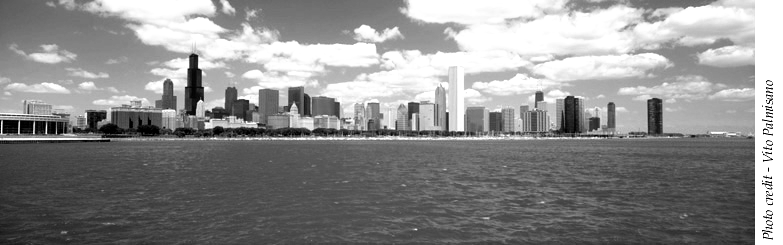
\includegraphics[width=\textwidth]{img/mmc_logo.png}
\end{titlepage}

\tableofcontents
	%\maketitle
\begin{centering}
	\date{\today}
\end{centering}
\newpage
\epigraph{There is only one large computer program I have used in which there are to a decent approximation 0 bugs: Don Knuth's TeX}{\textit{ -- Jaap Weel}}

\section{Getting Least Squares Line of Best Fit} % (fold)
\label{}
\subsection{From Calculator}
	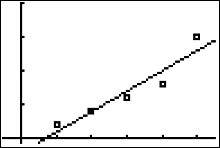
\includegraphics[width=.15\textwidth]{img/5_scat}

\subsection{From Summary Statistics} % (fold)
\label{sub:from_summary_statistics}
{\bf Formulas} (given): $\hat{y} = a + bx$\quad\quad$b = r\frac{s_y}{s_x}$\quad\quad$a=\bar{y}-b\bar{x}$\\[.2in]
{\bf Descriptive Statistics}: x, y\\
\verb|Variable  N  N*   Mean  SE Mean  StDev  Minimum     Q1  Median     Q3  Maximum|\\
\verb|x         5   0  3.000    0.707  1.581    1.000  1.500   3.000  4.500    5.000|\\
\verb|y         5   0   7.00     2.24   5.00     2.00   3.00    6.00  11.50    15.00|\\[.1in]
{\bf Correlations}: x, y \\
\verb|Pearson correlation of x and y = 0.949|\\
\verb|P-Value = 0.014|\\[.5in]

% subsection from_summary_statistics (end)

\subsection{From Output} % (fold)
\label{sub:from_output}
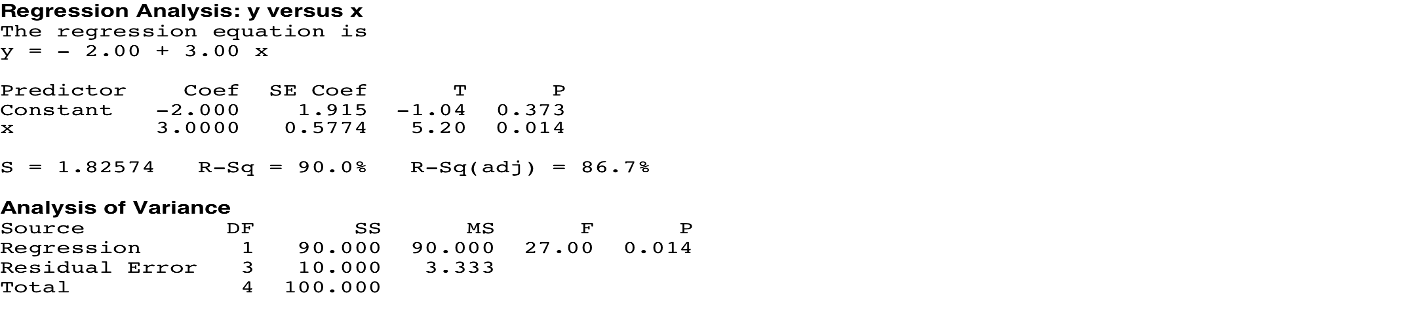
\includegraphics[width=1\textwidth]{img/5_RegOut}\\[.25in]

\subsection{Interpretation} % (fold)
\label{sub:interpretation}
\subsubsection{Slope}
Slope represents the  \textbf{predicted} change in response associated with each unit increase in the explanatory variable, \textbf{on average}.\\[.25in]
\subsubsection{Y-Intercept}
Y-intercept is the predicted value when the explanatory $(x)$ is 0. [Often the y-intercept is useless.]
% subsection interpretation (end)

\end{document}
